\documentclass[a4paper, 11pt]{article}
\usepackage[left=2cm,right=2cm,top=2cm,bottom=2cm]{geometry}
\usepackage{cite}
\usepackage{hyperref}
\usepackage{graphicx}

\title{From Flame to Inferno: A Literature Review of Cybersecurity Penetration Techniques}
\author{Jordan Peters}
\begin{document}


\begin{titlepage}
    \maketitle
    \begin{abstract}
        In 2010, a "worm" virus spread and embedded itself into approximately 100,000 systems and repeatedly malfunctioned 984 nuclear centrifuges over the span of at minimum 1 year, and likely more. It eluded detection by performing specific subroutines that would cause the equipment to only breakdown in such a way that it would cause no harm to people, and would make the scientists believe the equipment they were sold was just faulty and that they were unlucky.

        This virus was called Stuxnet, and its inception 10 years ago caused many researchers to become scared at the real-world implications that Stuxnet showed. Stuxnet proved that cybernetic attacks on critical infrastructures such as nuclear reactors are possible, and aren't just the type of attack that exists within the realms of theory or movie plotlines. Stuxnet was of such high complexity and danger that security researchers at Symantec said they hope to never see anything like this again.

        How do attacks like these ever get remotely close to the systems that they target? What are their routes of intrusion? Was it difficult for the attackers to attack this way, or is it easy if you have the knowhow? This literature review aims to answer the question of how cybersecurity penetration is often orchestrated, to finally demystify in an easily understandable way just how bad attacks like Stuxnet were, and how these horrors link back to software development. The hope is that this may educate developers to avoid practices that would lead software turning into husks for viruses like these before it is too late.
    \end{abstract}

    \begin{center}
    680041507

    I certify that all material in this dissertation which is not my own work has been identified.

    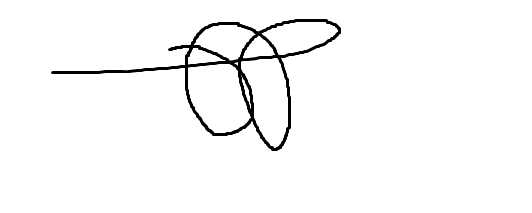
\includegraphics[width=200px]{figs/signature.png}

    \end{center}

\end{titlepage}

\tableofcontents


\pagebreak


\section{Introduction}
The security breach of a system is often the product of an incredibly complex thought up strategy \cite{ref:stuxnet2011report} that in some cases must be executed down to a T. With the goal usually being to deliver a "payload," a malicious program or section of malicious executed code on the victim computer, \cite{ref:singer2014cybersecurity} any number of vectors can be traversed to get the job done, but not all of them effective and not all of them the right option compared to another. 

Attack vectors, defined as the path used by an attacker to conduct an attack or to attempt to bypass system controls, \cite{ref:biometricattackvectors} are increasing as a result of new emerging technologies. \cite{ref:jang2014survey} As almost all of software developer's focus is put on developing software to solve a business problem, the security of this software becomes inherently neglected. The multi-contextual nature of software and its very large plethora of applications mean that the number of attack vectors attackers can choose to move through increase. These are commonly referred to in the same context as attack surfaces, known as the amount of ways an attacker can successfully attack a given system. \cite{ref:manadhata2010attack} The greater the attack surface, the more vulnerable the system.

This review covers, as comprehensive as practical, the amount of attack vectors that exist and are used today, and how they work in a non-cryptic way with otherwise actionable information to emphasise the importance of security flaws in software to software developers.

\section{Literature Review}
\subsection{Software Vulnerabilities}
\label{sec:softwarevul}
A combination of attack strategies are often used to accomplish a goal. Stuxnet uses zero-day vulnerabilities, through a type of attack vector known as software vulnerabilities, where mistakes in software code are exploited. \cite{ref:singer2014cybersecurity} For Stuxnet, vulnerabilities in antivirus software were exploited, along with system level vulnerabilities in Windows processes. During the virus' initial injection, it would scan the currently running antiviruses and system processes, read metadata like their version number, and decide which process to inject its malicious code into, optionally using one of two zero-day vulnerabilities for code injection that it contained. \cite{ref:stuxnet2011report} The virus does this to elevate privileges so it can perform any action it desires on the target computer. \cite{ref:stuxnet2011report} If no process was bypassable, the virus would become inert. \cite{ref:stuxnet2011report}

Exploiting vulnerabilities like this is the most common way of breaching the security of a system. \cite{ref:biometricattackvectors,ref:ibmbiometrics,ref:honeymoonsoftware} The question then becomes, how do attackers find these zero-day vulnerabilities?

At first glance it appears that zero-day vulnerabilities exist because developing large, complex software is hard and error prone. While this is invariably a factor, it dwarfs in comparison to other factors. Software enjoy a honeymood period, \cite{ref:honeymoonsoftware} coined the "Honeymoon Effect" in a study in 2010, where it was found that at the weakest point in a software's life cycle, its initial release, security vulnerabilities were never usually found during this period. It was described that an attacker's increasing familiarity with the software results in the discovery of the first zero-day way after the wave of ordinary bugs in software, where subsequent zero-days take less time to discover. Counterintuitively, the paper showed that code reuse, a strong development philosophy, was the greatest contributor to the rate and number of vulnerability discovery, which would otherwise suggest that to be the reason why large software (along with their popularity with users) are a strong target.

Attackers find vulnerabilities in software by approaching features of an application with certain expectations that typically arise from their programming experience. \cite{ref:sinstsipenyuk2005seven} talks of Adobe Reader 5.0 as an example, where failing to validate user supplied information causes an error called a "buffer overflow" to occur. A buffer overflow is where a program tries to store more data in a buffer than intended. \cite{ref:jang2014survey} The function (sprintf) that facilitated this overflow is only available in lower level languages such as C and C++, where lots of control is given to developers. Naturally, the ability to make these kinds of coding mistakes increases the more control is given to the developers as more things can go wrong. Input validation is an example of a "kingdom" among other "kingdoms" such as API abuse, encapsulation and poorly used security features, that are simply categories of mistakes that programmers make in software that open up abusable vulnerabilities. \cite{ref:sinstsipenyuk2005seven} An entire list of programming "sins" has been compiled alone to show how these common vulnerabilities easily manifest themselves within programs and what developers should look out for to stop them. \cite{ref:howardprogrammingsins200519} McGraw \cite{ref:mcgraw2004software} talks of the same vulnerabilities: error handling, buffer overflows, etc. but also notes that Internet-enabled software and the increasing extensibility of software add this greater fuel to the fire of increasing vulnerability. \cite{ref:sinstsipenyuk2005seven, ref:howardprogrammingsins200519} and \cite{ref:mcgraw2004software} have shown that developers, even in perhaps thought to be safer languages like Java and C\#, are creating common vulnerabilities in code every day, and \cite{ref:honeymoonsoftware} shows that code reuse only makes it worse as developers are under the falsehood that the code is safer and more reliable due to its maturity. To conclude the mystery of software vulnerability exploitation, \cite{ref:sinstsipenyuk2005seven,ref:honeymoonsoftware,ref:howardprogrammingsins200519,ref:mcgraw2004software,ref:biometricattackvectors,ref:stuxnet2011report} demonstrate that attackers reverse engineer large, popular and complex software, scanning for common security vulnerabilities in every major update of these software. They discover these lingering zero-day exploits and sell them on the market \cite{ref:jang2014survey} to the highest bidder, or stockpile for use themselves in attacks such as with Stuxnet \cite{ref:stuxnet2011report}.

\subsection{Internet of Things}
\label{sec:iot}
The advent of the Internet of Things (IoT) has revolutionized many physical devices today. Replay attacks are an example of an attack against IoT devices that could, for example, allow you to turn off a lightbulb using a custom made program and a repurposed HTTP request that was sent before your one. Or, you could deliver a deadly, 830-volt shock to a victim's pacemaker from up to 50 feet away using a laptop. \cite{ref:pacemakers} The previous fact was not a lie: the network traffic between some pacemakers and the Internet are unencrypted. \cite{ref:pacemakers} This one simple security flaw allows all traffic between the pacemaker and the Internet to be not only viewed, but modified and replayed at will, and is a quintessential scenario for replay attacks. Since 2017 when the paper was written, pacemakers were still operating with this security vulnerability.

\subsection{Spoofing Biometric Systems}
\label{sec:spoofingbiometric}
The most prominent method of circumventing biometric systems, such as fingerprint scanners, iris scanners and facial recognition devices, is spoofing. \cite{ref:biometricattackvectors} Spoofing is the presentation of an item, false data or a false biometric claiming to be legitimate, resulting in a system triggering a false positive and granting access. \cite{ref:biometricattackvectors}

What some might consider to be reserved to James Bond movies is very much practical in real life. For example, the most basic form of spoofing appears to be lifting fingerprints and re-using them, which began research back in 1998. \cite{ref:biometricattackvectors,ref:willis1998six} They found that 4 out of 6 devices tested were susceptible to these fake finger attacks. \cite{ref:willis1998six}

The next step up was the use of "gummy fingers" in 2002 \cite{ref:matsumoto2002impact}, where finger sleeves were made from gelatine and fingerprints were imprinted on them. Their research showed a high acceptance rate from fingerprint readers that used optical (measuring the reflection of light \cite{ref:matsumoto2002impact}) or capacitative (the ability for something to store electrical charge) sensors, which were most fingerprint readers back then. \cite{ref:matsumoto2002impact}

Then two German hackers in August 2003 claimed to have developed a technique of using prints left behind on a scanner and converting them into a latex finger, reconstructing digital images of the prints left behind on scanners into three-dimensional replications of the fingerprint. \cite{ref:biometricattackvectors,ref:harrison2003hackers} The reliability of this information is called into question however. While discovered from \cite{ref:biometricattackvectors} with 275 citations from this time of reading (1st March 2020), the source that article got it from \cite{ref:harrison2003hackers} is from a website called Security Focus in 2003 with 7 citations. Further information or proof of the proceedings that \cite{ref:harrison2003hackers} describes are incomplete.

Other methods include playing back digital videos or images into iris sensors and facial recognition to gain access \cite{ref:bodybiometrie,ref:biometricattackvectors}, where some demonstrations of attacking this way even included poking a hole in a photograph of an iris to trick the 'liveness' testing mechanism inside some iris sensors. Liveness is the primary security mechanism to counter spoofing. Put simply, liveness involves seeing whether whatever is being sensed is actually alive. \cite{ref:biometricattackvectors}

\subsection{Collusion and Coercion}
\label{sec:coercion}
The threat of being exposed for some sort of secret is a very effective motivator to make someone do something for you, such as giving up their biometric and access privileges \cite{ref:biometricattackvectors} or inserting removable drives that carry a payload into a confidential system for you. The reputation of a person can be damaged beyond repair with the right allegation, making this style of attack vector very powerful but difficult to pull off.

However, coercion doesn't have to be voluntary. Being tricked into opening infected files, being lured into visiting a malware propagating website (\ref{sec:driveby}) or having your login details stolen from an attacker's authentic-looking page (\ref{sec:phishing}) are all forms of involuntary coercion \cite{ref:jang2014survey,ref:singer2014cybersecurity}, a promising attack vector. \cite{ref:biometricattackvectors} and \cite{ref:jang2014survey} both show that using people as a weapon can open up many vectors of attack within an organization, with both falling under the area of social engineering, described by Singer \cite{ref:singer2014cybersecurity} as the manipulation of people in revealing confidential information and helping an attacker.

\subsection{Phishing}
\label{sec:phishing}
Phishing is a form of social engineering (\ref{sec:coercion}) where an attacker fraudently acquires information from a victim by impersonating as a legitimate third party. \cite{ref:phishing} The attack vectors of phishing are very broad, but each one revolves around a core theme: social networks. By data mining social media websites, it's easy to send out spam messages to people. \cite{ref:phishing} The paper even describes context aware phishing, where, for example, an attacker could login to a victim's account incorrectly so many times that it becomes locked. The attacker could follow up with an email impersonating the website offering to help the victim as a result of what happened, unknowingly coercing the victim into the attacker's trap. Phishing as an attack vector revolves around building and exploiting the trust with a victim. \cite{ref:phishing} discusses many intelligent ways that publicly accessible information can be mined and re-used in messages to the victim to trick them and to build trust with them. 

\subsection{Browser Extensions}
\label{sec:extensions}
While most people don't think too much about what allowing permissions for browser extensions actually does, the potential for browser extensions as an attack vector to spread a payload such as a botnet is a profoundly effective strategy. Many security flaws are present in browsers \cite{ref:reis2009browser, ref:soghoian2007remote}. Although Google Chrome attempts to sandbox as much as it can, it cannot do this perfectly. Certain extensions like Silverlight that allow feature-rich usage on websites must be used and are not designed to be in a sandboxed environnment. \cite{ref:reis2009browser}

More topically, a browser extension called Web of Trust logged and sold the data of all web requests to third parties. \cite{ref:brucker2017evil} When a German TV station bought this data and de-anonymized it, details about international search warrants and the tax declarations of members of parliament were revealed. \cite{ref:brucker2017evil} One extension even replaced phone numbers for security firms with their own malicious phone numbers in an attempt to masquerade as these firms and phish (\ref{sec:phishing}) users unknowingly in times of need.

\subsection{Driveby}
\label{sec:driveby}
Driveby attacks were a prevalent topic in 2008 \cite{ref:kanich2008spamalytics} where the 'Storm' worm virus had been reverse engineered and experimented with to document its behaviour. This attack vector is simple. A website, when a user lands on it, automatically downloads malware to a user's computer. If the user installs the program, usually acting as some innocuous program, the payload will activate. In Storm's case, this would attach the user to a botnet and propagate the malware across a user's entire address book, causing further drivebys along the way.

\subsection{Botnet}
\label{sec:botnet}
Botnets are a special type of payload propagation, where Koobface, a great example of a botnet-propagated payload spread across social network accounts and turned accounts into "zombies," spreading spam links that friends of a user would click and in turn be enslaved. \cite{ref:thomas2010koobface} Intelligently, the malware prompts a user to install a flash executable after going through several steps that get the user into the right location inconspicuously. If the user says yes, the user becomes a new zombie and is attached to this botnet. Attackers will often continually compromise new domains as hosts get taken down, where 323 hosts were compromised to act as transient command and control servers at any time with an average of 97 always running despite them being taken down.

\subsection{Smartphones}
\label{sec:smartphones}
As demonstrated in \ref{sec:softwarevul}, the rapid emergence of technologies and reuse of existing code to accomplish this has made the rate of vulnerability exploitation skyrocket. \cite{ref:jang2014survey} Smartphones are naturally a fulcrum of this problem, with huge market demand forcing these phones to integrate multiple wireless networking technologies to support new features and services. \cite{ref:mulliner2006security} Significant amounts of new firmware and hardware models are released every year, and a major focus on new features and the neglecting of security has made smartphones a bright target for attackers. \cite{ref:mulliner2006security} As Mulliner \cite{ref:mulliner2006security} puts it, smart phones now face new security problems not found elsewhere.

One of these such problems was resident in some of the mobile's software. Its web browser for instance had a buffer overflow vulnerability, which via the exploitation of a regular expression parser for WebKit in Apple's Safari, managed to cause an overflow and execution of the arbitrary code injected from a web page. \cite{ref:dunham2008mobile} This allowed every iPhone in existence at the time to be jailbroken just by visiting a website.

On the attack vector front, Bluetooth comes to mind. In 2006 there had been no viruses that exploited actual vulnerabilities in Bluetooth, but these vulnerabilties do exist, they just require custom hardware and would appear to be impractical as a virus. \cite{ref:toyssy2006malicious} Most examples of viruses via this transmission required significant user input. For example, users would need to turn on their Bluetooth, and then accept the file manually for the payload to execute. If wireless or wireless local area network (WLAN) abilities become more commonplace, like they have today compared to 2006, it was hypothesised that viruses will probably use these as an attack vector as well. \cite{ref:toyssy2006malicious}

\subsection{Cloud computing}
Cloud computing is a fantastic addition to the modern world that makes cloud data storage for companies small and big seamless, scalable and easy to use. \cite{ref:jang2014survey} Naturally however this means clients need to put their full trust in cloud providers to keep their data fully secure and untampered \cite{ref:zhang2010cloud} with, and these cloud providers have to trust in the infrastructure providers to deal with the requests required of the data. Due to the virtual nature of servers within the cloud, that is to say, the fact that they can move at any time, it's increasingly difficult to be able to create an entirely trusted policy that works all the way from the hardware layer and up that will keep data confidential and auditable, where auditable means that the security settings chosen by a client and forwarded by a cloud provider have not been changed, and that system logs cannot be tampered with. \cite{ref:zhang2010cloud} Creating this trusted system that works well with a customer's ever-evolving behaviours and the elastic nature of the cloud is an active area of research today.

\section{Conclusion}
By far, the most powerful strategy for attackers is to first discover, then exploit software vulnerabilities, and then use social engineering to make people download and execute their payload. The ways this strategy can manifest itself however is rapidly increasing every day - with the advent of IoT personal and medical devices, cloud computing and smartphones, the amount of ways someone can attack a person or organization are scary to consider. \cite{ref:honeymoonsoftware,ref:sinstsipenyuk2005seven,ref:mcgraw2004software,ref:howardprogrammingsins200519} show that all software today, from the operating system, to the web browsers, messaging services and tools we use every day have hidden zero-day vulnerabilities inside all of them. As future software developers who will work on large commercial applications, it is clear it is imperative to understand both how to engineer quality software \bfseries and \mdseries develop secure software. Ignoring this presents a revelling catastrophe of the likes of Stuxnet \cite{ref:stuxnet2011report}, but likely worse. Further reading and research should reach further into how software can be tested for vulnerability and how we can design software from the ground up to be resistant or effectively clear of vulnerability altogether.

\section{Bibliography}
\bibliographystyle{IEEEtran}
\bibliography{references}

\end{document}